Im Rahmen dieses Projekts fungiert Docker als primäre Technologie für die
Containerisierung der entwickelten Anwendung. Das Hauptziel besteht darin,
eine homogene und wiederholbare Ausführungsumgebung für sämtliche
Systemkomponenten zu etablieren. Der Docker-Einsatz ermöglicht die
konsistente Gestaltung von Entwicklungs- und Produktivumgebungen, wodurch
potenzielle Fehlerquellen durch divergierende Systemkonfigurationen
deutlich reduziert werden.

Das System setzt sich aus mehreren funktional abgegrenzten Komponenten
zusammen, die jeweils dedizierte Funktionen erfüllen. Hierzu gehören eine
Benutzeroberfläche für die Interaktion mit Anwendern, ein Backend für die
Abwicklung der Geschäftslogik sowie ergänzende Services wie ein
Datenbanksystem. Diese Komponenten werden in eigenständigen Containern
betrieben, was eine präzise Aufgabentrennung realisiert.

\begin{figure}[H]
    \centering
    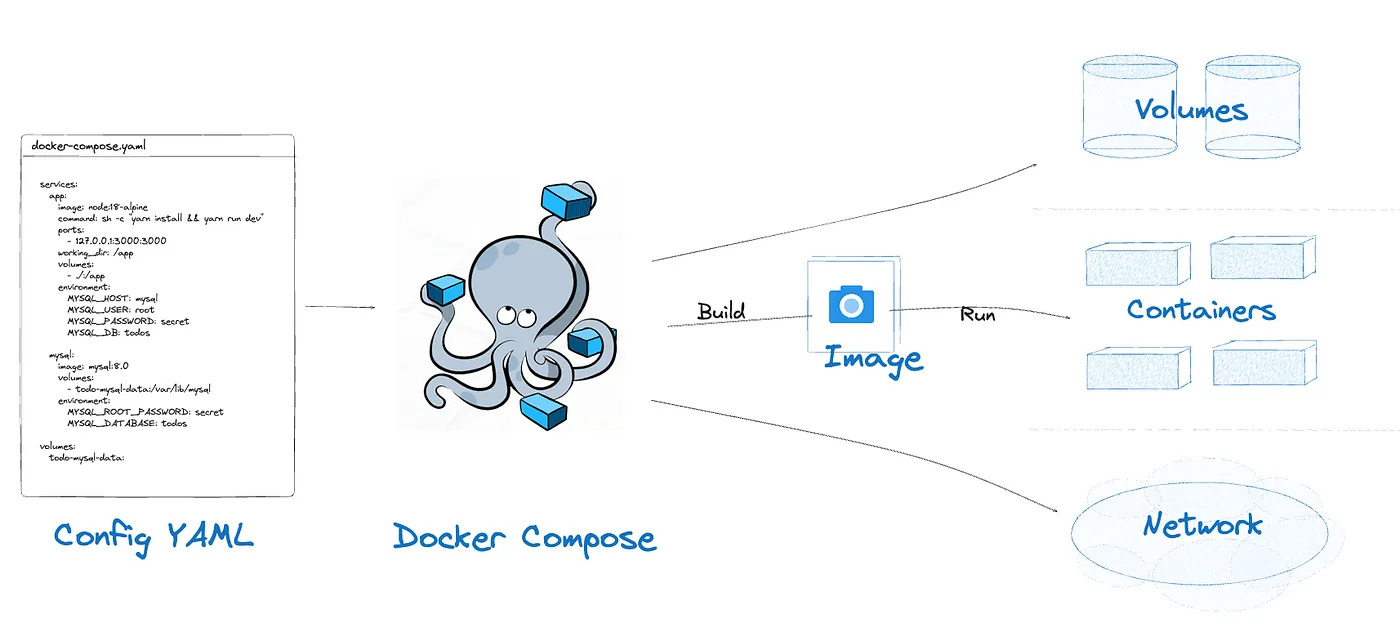
\includegraphics[width=0.9\textwidth]{pics/docker_compose.jpg}
    \caption{Architektur der containerisierten Anwendung im Projekt}
    \label{fig:docker-projekt-architektur}
\end{figure}

Abbildung~\ref{fig:docker-projekt-architektur} veranschaulicht die
grundsätzliche Struktur der containerisierten Projektarchitektur. Die
einzelnen Container operieren innerhalb der Docker Engine und tauschen
Informationen über ein internes virtuelles Netzwerk aus. Der Zugang von
außen erfolgt ausschließlich über festgelegte Schnittstellen, wodurch eine
geregelte und abgesicherte Kommunikation sichergestellt wird.

Ein bedeutender Nutzen dieser Architektur manifestiert sich in ihrer
Modularität. Modifikationen an einzelnen Komponenten, etwa der
Benutzeroberfläche, lassen sich realisieren, ohne dass andere Systemteile
davon betroffen sind. Zusätzlich können individuelle Container autonom
neugestartet oder aktualisiert werden, was Wartungsoperationen erleichtert.

Docker bietet darüber hinaus die Möglichkeit, Abhängigkeiten explizit
innerhalb der jeweiligen Container zu spezifizieren. Dies macht die
Installation bestimmter Softwareversionen oder Laufzeitumgebungen direkt
auf dem Host-System überflüssig. Die Anwendung wird stattdessen vollständig
durch die Container-Images charakterisiert, was die Transparenz und
Reproduzierbarkeit des Deployment-Prozesses steigert \cite{dockerdocs}.

Für den Entwicklungsablauf ergibt sich durch Docker ein zusätzlicher Vorzug:
Neue Projektmitglieder können mit minimalem Konfigurationsaufwand mit der
Arbeit beginnen. Durch das Bauen der Container-Images und den Start der
Container entsteht unmittelbar eine funktionsfähige Umgebung, ohne dass
händische Einrichtungsschritte notwendig werden.

Zusammenfassend bildet Docker im Projekt ein fundamentales Element zur
Realisierung einer strukturierten, wartungsfreundlichen und zukunftsfähigen
Systemarchitektur. Die eindeutige Separation der einzelnen Services sowie
die einheitliche Laufzeitumgebung schaffen das Fundament für die
nachfolgenden Schritte der Container-Konfiguration, die in den
anschließenden Abschnitten detailliert beschrieben werden.